\documentclass[letterpaper]{article}
\usepackage[margin=1in]{geometry}
\usepackage[utf8]{inputenc}
\usepackage{textcomp}
\usepackage{amssymb}
\usepackage{natbib}
\usepackage{graphicx}
\usepackage{gensymb}
\usepackage{amsthm, amsmath, mathtools}
\usepackage[dvipsnames]{xcolor}
\usepackage{enumerate}
\usepackage{mdframed}
\usepackage[most]{tcolorbox}
\usepackage{csquotes}
% https://tex.stackexchange.com/questions/13506/how-to-continue-the-framed-text-box-on-multiple-pages

\tcbuselibrary{theorems}

\newcommand{\R}{\mathbb{R}}
\newcommand{\Z}{\mathbb{Z}}
\newcommand{\N}{\mathbb{N}}
\newcommand{\Q}{\mathbb{Q}}
\newcommand{\C}{\mathbb{C}}
\newcommand{\code}[1]{\texttt{#1}}
\newcommand{\mdiamond}{$\diamondsuit$}
\newcommand{\PowerSet}{\mathcal{P}}
\newcommand{\Mod}[1]{\ (\mathrm{mod}\ #1)}
\DeclareMathOperator{\lcm}{lcm}

%\newtheorem*{theorem}{Theorem}
%\newtheorem*{definition}{Definition}
%\newtheorem*{corollary}{Corollary}
%\newtheorem*{lemma}{Lemma}
\newtheorem*{proposition}{Proposition}


\newtcbtheorem[number within=section]{theorem}{Theorem}
{colback=green!5,colframe=green!35!black,fonttitle=\bfseries}{th}

\newtcbtheorem[number within=section]{definition}{Definition}
{colback=blue!5,colframe=blue!35!black,fonttitle=\bfseries}{def}

\newtcbtheorem[number within=section]{corollary}{Corollary}
{colback=yellow!5,colframe=yellow!35!black,fonttitle=\bfseries}{cor}

\newtcbtheorem[number within=section]{lemma}{Lemma}
{colback=red!5,colframe=red!35!black,fonttitle=\bfseries}{lem}

\newtcbtheorem[number within=section]{example}{Example}
{colback=white!5,colframe=white!35!black,fonttitle=\bfseries}{def}

\newtcbtheorem[number within=section]{note}{Important Note}{
        enhanced,
        sharp corners,
        attach boxed title to top left={
            xshift=-1mm,
            yshift=-5mm,
            yshifttext=-1mm
        },
        top=1.5em,
        colback=white,
        colframe=black,
        fonttitle=\bfseries,
        boxed title style={
            sharp corners,
            size=small,
            colback=red!75!black,
            colframe=red!75!black,
        } 
    }{impnote}
\usepackage[utf8]{inputenc}
\usepackage[english]{babel}
\usepackage{fancyhdr}
\usepackage[hidelinks]{hyperref}

\pagestyle{fancy}
\fancyhf{}
\rhead{CSE 105}
\chead{Wednesday, January 12, 2022}
\lhead{Lecture 4}
\rfoot{\thepage}

\setlength{\parindent}{0pt}

\begin{document}

\section{The Regular Operations (Continued)}
We will review some of the regular operations. 

\subsection{Concatenation}
Recall that concatenation is defined by: 
\[A \circ B = \{xy \mid x \in A \text{ and } y \in B\}\]
How would this works for $A = \{a^n \mid n \geq 0\}$ and $B = \{b^m \mid m \geq 0\}$?
\[A \circ B = \{a^n b^m \mid n, m \geq 0\}\]
We can use NFAs to show that this is the case. 

\section{Nondeterministic Finite Automata (1.2)}
In a deterministic finite automata, when the machine was in a given state and reads the next input symbol, we knew that the next state is; that's why it's called \emph{determinstic}, because it was already determined. \textbf{However}, in a \emph{nondeterministic} machine, several choices may exist for the next state at any point. In general, nondeterminism is a \emph{generalization} of determinism; that is, every deterministic finite automaton is automatically a nondeterminism finite automaton.

\subsection{The Differences Between DFA and NFA}
\begin{center}
    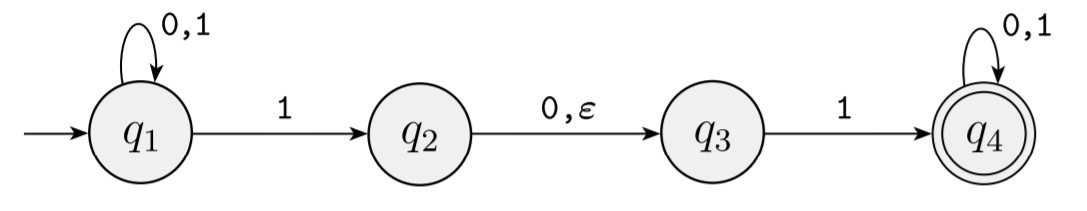
\includegraphics[scale=0.4]{../assets/nfa_1.png}
    
    \textbf{Figure:} The nondeterministic finite automaton $N_1$. 
\end{center}

\begin{center}
    \begin{tabular}{p{3in}|p{3in}}
        \textbf{DFA} & \textbf{NFA} \\ 
        \hline 
        \begin{itemize}
            \item Every state of a DFA always has exactly one exiting transition arrow for each symbol in the alphabet.
            \item There is a unique computation path for each input. 
            \item Labels on the transition arrows are symbols from the alphabet. 
        \end{itemize} 

        & \begin{itemize}
            \item Not every state in an NFA needs exactly one transition arrow for each symbol. In an NFA, a state may have zero, one, or many exiting arrows for each alphabet symbol.
            \item We may allow several (or zero) alternative computations on the same input. 
            \item NFAs may have arrows labeled with members of the alphabet or $\epsilon$. Zero, one, or many arrows may exit from each state with the label $\epsilon$. For example, the above figure has one transition arrow with $\epsilon$ as a label. 
        \end{itemize}
    \end{tabular}
\end{center}

\subsection{NFA Computation}
How does an NFA compute? Suppose that we are running an NFA on an input string and come to a state with multiple ways to proceed. Suppose, in fact, that we use the NFA above: $N_1$. Additionally, suppose that we are at state $q_1$, and the next input symbol is \code{1}. 
\begin{itemize}
    \item After reading this symbol, the machine \textbf{splits into multiple copies of itself} and follows \emph{all} the possibilities in \emph{parallel}. In other words, each copy of the machine takes one of the possible ways to proceed and continues as before. 
    \item If there are subsequent choices, the machine splits again. 
    \item If the next input symbol doesn't appear on any of the arrows exiting the stae occupied by a copy of the machine, that copy of the machine dies.
    \item If any one of these copies of the machine is in an accept state at the \underline{end of the input}, the NFA \emph{accepts} the input string.
\end{itemize}
What happens when we come across a state with an $\epsilon$ symbol on an exiting arrow? Well, without reading any input, the machine splits into \emph{multiple} copies, one following each of the exiting $\epsilon$-labeled arrows and one staying at the current state. The machine, then, proceeds nondeterministically as before. So, really, $\epsilon$ transitions allow the machine to \textbf{transition between states spontaneously} without consuming any input symbols.

\begin{center}
    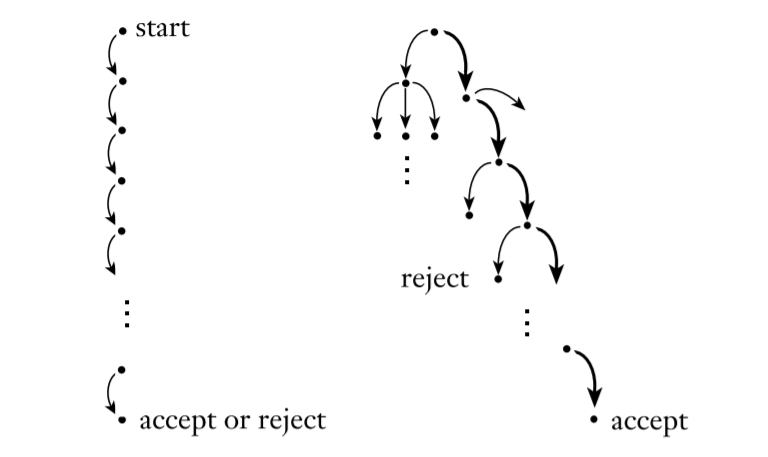
\includegraphics[scale=0.4]{../assets/nfa_vs_dfa.png}

    \textbf{Figure:} Difference between deterministic computation and nondeterministic computation. 
\end{center}

We can see nondeterminism as some kind of parallel computation, where multiple independent ``threads'' or ``processes'' can be started concurrently. Whenever the NFA splits to follow several choices, that corresponds to a process ``forking'' into several children, of which each proceeds separately. Also, if one of the processes accepts, the entire computation accepts. 


\subsection{Formal Definition of NFA}
The formal definition of a nondeterministic finitne automaton is essentially the same as the one for a deterministic finitne automaton. The major difference, though, is the transition function. In particular:
\begin{center}
    \begin{tabular}{p{3in}|p{3in}}
        \textbf{DFA} & \textbf{NFA} \\ 
        \hline 
        The transition function takes a state and an input symbol, and produces the next state. & The transition function takes a state and an input symbol \emph{or} the empty string, and produces the \emph{set of possible next states}.
    \end{tabular}
\end{center}

With this in mind, we consider the definition:
\begin{definition}{Nondeterministic Finite Automaton}{}
    A \textbf{nondeterministic finite automaton} is a 5-tuple $(Q, \Sigma, \delta, q_0, F)$ where: 
    \begin{enumerate}
        \item $Q$ is a finite set called the \textbf{states}.
        \item $\Sigma$ is a finite set called the \textbf{alphabet}.
        \item $\delta: Q \times \Sigma \cup \{\epsilon\} \mapsto \PowerSet(Q)$ is the \textbf{transition function}.
        \item $q_0 \in Q$ is the \textbf{start state}.
        \item $F \subseteq Q$ is the \textbf{set of accept states} (sometimes also called \emph{final states}).
    \end{enumerate}
\end{definition}
\textbf{Remarks:}
\begin{itemize}
    \item $\Sigma \cup \{\epsilon\}$ is sometimes written as $\Sigma_{\epsilon}$.
    \item We say that $\delta(q, c)$ returns a \textbf{set} of states; more precisely, a subset of $Q$. Here, $c \in \Sigma$ or $\epsilon$ and $q \in Q$.
\end{itemize}

\subsubsection{Example: Starting NFA}
Recall the NFA $N_1$:
\begin{center}
    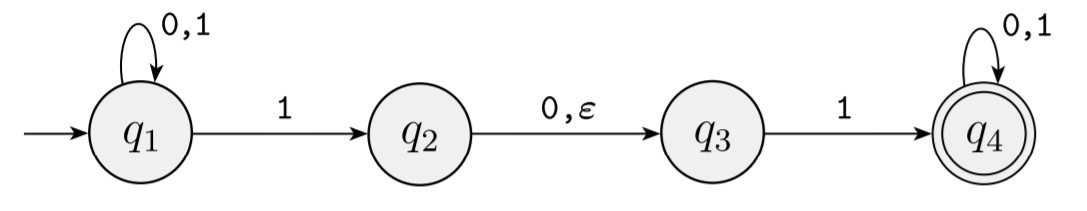
\includegraphics[scale=0.4]{../assets/nfa_1.png}
\end{center}
Here, the formal description of $N_1$ is given by: 
\begin{itemize}
    \item $Q = \{q_1, q_2, q_3, q_4\}$
    \item $\Sigma = \{\code{0}, \code{1}\}$
    \item $\delta$ is given as:
    \begin{center}
        \begin{tabular}{c|c c c}
                  & \code{0} & \code{1} & $\epsilon$ \\ 
            \hline 
            $q_1$ & $\{q_1\}$ & $\{q_1, q_2\}$ & $\emptyset$ \\ 
            $q_2$ & $\{q_3\}$ & $\emptyset$ & $\{q_3\}$ \\ 
            $q_3$ & $\emptyset$ & $\{q_4\}$ & $\emptyset$ \\ 
            $q_4$ & $\{q_4\}$ & $\{q_4\}$ & $\emptyset$
        \end{tabular}
    \end{center}
    \item $q_1$ is the start state
    \item $F = \{q_4\}$
\end{itemize}

\subsection{Acceptance in an NFA}
We say that an NFA $(Q, \Sigma, \delta, q_0, F)$ accepts a string $w$ in $\Sigma^*$ if and only if we can write $w = y_1 y_2 \dots y_m$ where each $y_i \in \Sigma_{\epsilon}$ and there is a sequence of states $r_0, \dots, r_m \in Q$ such that: 
\begin{enumerate}
    \item $r_0 = q_0$. The machine starts in the start state. 
    \item $r_{i + 1} \in \delta(r_i, y_{i + 1})$ for each $i = 0, 1, \dots, m - 1$. The state $r_{i + 1}$ is one of the allowable next states when $N$ is in state $r_i$ and reading $y_{i + 1}$. Here, we note that $\delta(r_i, y_{i + 1})$ is the set of allowable next states.  
    \item $r_m \in F$. The machine accepts its input if the last state is an accept state. 
\end{enumerate}

\end{document}